\documentclass[aspectratio=169,11pt]{beamer}

\usepackage[utf8]{inputenc}
\usepackage[T1]{fontenc}
\usepackage[spanish]{babel}
\usepackage{booktabs}
\usepackage{array}
\usepackage{graphicx}
\usepackage{xcolor}
\usepackage{amssymb}

\graphicspath{{Paper/figures/}{figures/}}

\definecolor{cjcblue}{HTML}{1F5EA8}
\definecolor{cjcyellow}{HTML}{F2C400}
\definecolor{cjcgray}{HTML}{4A4A4A}
\definecolor{cjclight}{HTML}{F5F6F7}

\usetheme{default}
\setbeamertemplate{navigation symbols}{}
\setbeamertemplate{footline}{
  \leavevmode%
  \hbox{%
    \begin{beamercolorbox}[wd=.78\paperwidth,ht=2.4ex,dp=1.1ex,leftskip=1.5em]{author in head/foot}%
      \scriptsize Centro Javeriano de Competitividad
    \end{beamercolorbox}%
    \begin{beamercolorbox}[wd=.22\paperwidth,ht=2.4ex,dp=1.1ex,rightskip=1.5em plus1fil]{date in head/foot}%
      \scriptsize \insertframenumber/\inserttotalframenumber
    \end{beamercolorbox}}%
  \vskip0pt%
}

\setbeamercolor{frametitle}{fg=cjcblue}
\setbeamercolor{title}{fg=cjcblue}
\setbeamercolor{normal text}{fg=black,bg=white}
\setbeamercolor{author in head/foot}{fg=white,bg=cjcblue}
\setbeamercolor{date in head/foot}{fg=white,bg=cjcgray}
\setbeamerfont{frametitle}{series=\bfseries,size=\large}
\setbeamerfont{title}{series=\bfseries,size=\LARGE}
\setbeamertemplate{itemize item}{\color{cjcblue}$\blacktriangleright$}
\setbeamertemplate{itemize subitem}{\color{cjcblue}$\bullet$}

\newcommand{\fuente}[1]{\vspace{0.15cm}{\tiny\color{cjcgray}#1}}
\newcommand{\idea}[1]{\textbf{\color{cjcblue}#1}}
\newcommand{\cjcbar}{\textcolor{cjcyellow}{\rule{0.18\textwidth}{1.6pt}}\hspace{0.3em}\textcolor{cjcblue}{\rule{0.72\textwidth}{1.6pt}}}
\newcommand{\subactividadfuente}{\fuente{Nota: PIB/trab. 2025 en millones de pesos constantes de 2015; PIB/hora 2025 en miles de pesos constantes de 2015. Fuente: cálculos propios con DANE y GEIH.}}
\newcommand{\trayectoriaframe}[1]{%
  \begin{frame}{Trayectoria anual de la productividad}
    \begin{center}
      \includegraphics[width=0.98\textwidth,height=0.78\textheight,keepaspectratio]{presentation_panels/fig_presentacion_indices_#1.png}
    \end{center}
    \fuente{Fuente: cálculos propios con DANE y GEIH.}
  \end{frame}
}
\newcommand{\descomposicionframe}[1]{%
  \begin{frame}{Descomposición del crecimiento por actividad}
    \begin{center}
      \includegraphics[width=0.98\textwidth,height=0.78\textheight,keepaspectratio]{presentation_panels/fig_presentacion_descomposicion_#1.png}
    \end{center}
    \fuente{Fuente: cálculos propios con DANE y GEIH.}
  \end{frame}
}

\title{Dinámicas de la Productividad Laboral por Actividad Económica en Colombia, 2010--2025}
\subtitle{Informes sobre la Productividad en Colombia \\ Informe 01}
\author{Oliver Pardo \and Jorge Orozco}
\institute{Centro Javeriano de Competitividad}
\date{Junio de 2026}

\begin{document}

\begin{frame}[plain]
  \vspace{0.3cm}
  
\includegraphics[height=1.45cm]{logo_cjc_palatino_horizontal.png}

  \vspace{0.8cm}
  {\Large\color{cjcgray}Informes sobre la Productividad en Colombia}\\[0.2cm]
  {\large\color{cjcgray}Informe 01}\\[0.35cm]
  \cjcbar

  \vspace{0.8cm}
  {\LARGE\bfseries\color{cjcblue} Dinámicas de la Productividad Laboral por Actividad Económica en Colombia, 2010--2025}

  \vfill
  {\large Oliver Pardo \quad | \quad Jorge Orozco}\\[0.15cm]
%  {\normalsize Centro Javeriano de Competitividad}\\[0.1cm]
  {\normalsize Junio de 2026}
\end{frame}

\begin{frame}{Motivación de la serie}
  \idea{Los Informes sobre la Productividad en Colombia buscan convertir la productividad en una conversación pública informada y útil para la toma de decisiones.}

  \vspace{0.4cm}
  \begin{itemize}
    \item La productividad no es solo un dato que se observa: también es resultado de políticas públicas, decisiones de inversión, adopción tecnológica y organización empresarial.
    \item La serie combina distintas fuentes de información para medir cómo evoluciona la productividad en el agregado, entre actividades económicas, entre territorios y entre grupos de trabajadores.
    \item El objetivo es identificar dónde están los rezagos, dónde hay avances y qué preguntas debe responder una agenda nacional de productividad.
  \end{itemize}
\end{frame}

\begin{frame}{Por qué importa la productividad laboral}
  \idea{Colombia no puede depender indefinidamente de incorporar más personas al mercado laboral para elevar el ingreso promedio.}

  \vspace{0.4cm}
  \begin{itemize}
    \item El crecimiento del ingreso por habitante depende de cuántas personas trabajan y de cuánto produce cada trabajador.
    \item En una sociedad que envejece, el margen para crecer solo con más ocupados será cada vez menor.
    \item Por eso, la productividad laboral debe ser una prioridad de la agenda económica: no solo se mide, también se construye con políticas públicas.
  \end{itemize}
\end{frame}

\begin{frame}{Qué mide el informe}
  \idea{El informe combina cuentas nacionales y GEIH para medir el producto por trabajador y el producto por hora trabajada.}

  \vspace{0.45cm}
  \begin{block}{Descomposición básica}
    \[
      PIB = Ocupados \times \frac{Horas}{Ocupados} \times \frac{PIB}{Horas}
    \]
  \end{block}

  \vspace{0.25cm}
  \begin{itemize}
    \item El PIB y el valor agregado por actividad económica provienen de las cuentas nacionales del DANE.
    \item Los ocupados y las horas trabajadas se calculan con la GEIH como promedios anuales.
    \item El periodo de análisis es 2010--2025 y los valores monetarios están expresados en pesos constantes de 2015.
  \end{itemize}
\end{frame}

\begin{frame}{El panorama agregado}
  \idea{Entre 2010 y 2025, el PIB real creció 3,16\% anual, pero el PIB por trabajador aumentó apenas 1,05\% anual.}

  \vspace{0.25cm}
  \begin{center}
  \small
  \begin{tabular}{lrrr}
    \toprule
    Indicador & 2010 & 2025 & Crec. anual \\
    \midrule
    PIB real (Billones de pesos de 2015) & 640 & 1.021 & 3,16\% \\
    Ocupados (Millones) & 16,8 & 23,0 & 2,09\% \\
    PIB por trabajador (Millones de pesos de 2015) & 38,0 & 44,5 & 1,05\% \\
    Horas semanales por trabajador & 46,8 & 43,7 & -0,45\% \\
    PIB por hora trabajada (Miles de pesos de 2015) & 15,6 & 19,6 & 1,51\% \\
    \bottomrule
  \end{tabular}
  \end{center}

  \fuente{Fuente: cálculos propios con base en Cuentas Nacionales y GEIH del DANE.}
\end{frame}

\begin{frame}{De dónde salió el crecimiento del PIB}
  \idea{El crecimiento del PIB fue impulsado por más ocupados y por mayor producto por hora, mientras que las horas por trabajador cayeron.}

  \vspace{0.2cm}
  \begin{center}
    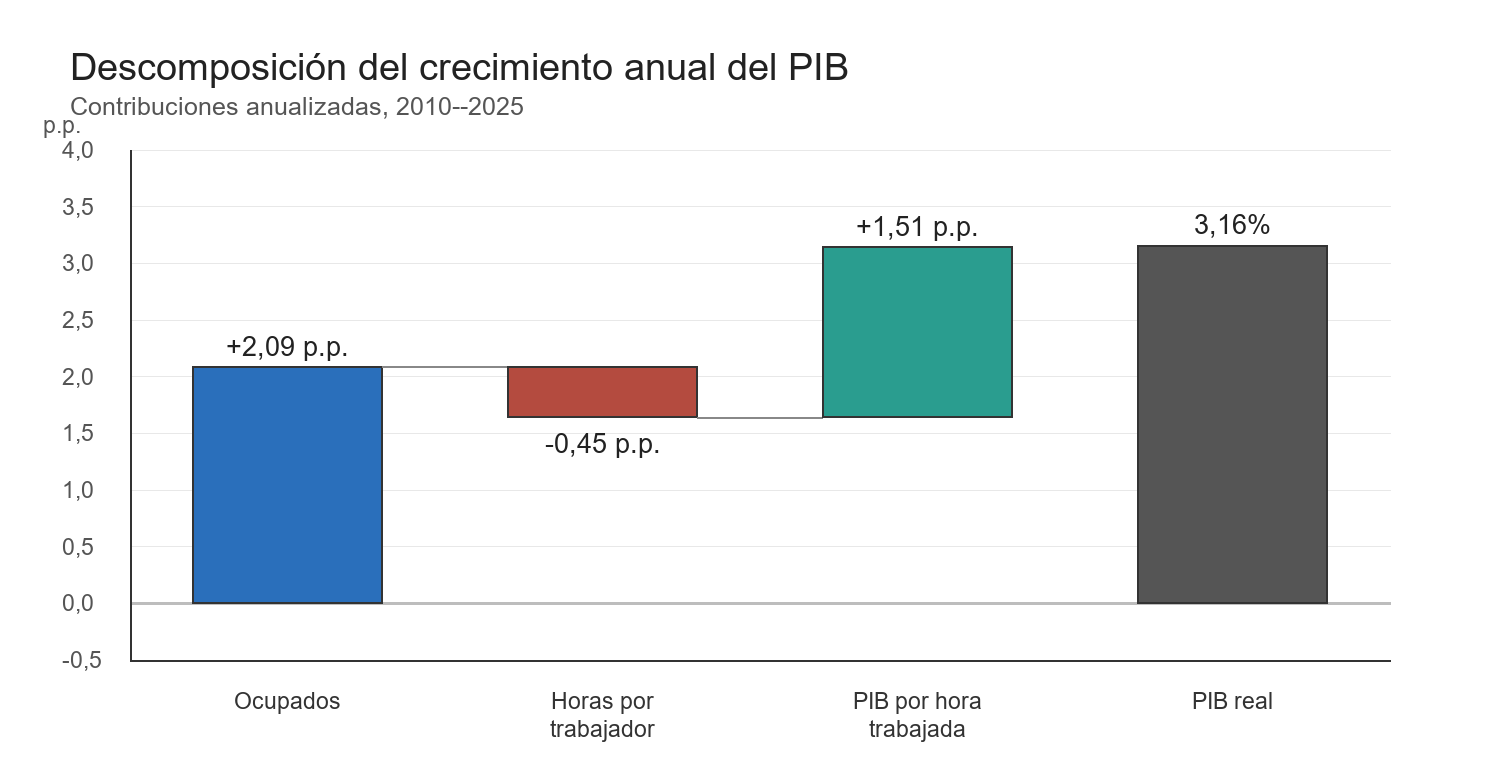
\includegraphics[width=0.86\textwidth,height=0.67\textheight,keepaspectratio]{fig_pib_geih_descomposicion_crecimiento.png}
  \end{center}

  \fuente{Fuente: cálculos propios con base en Cuentas Nacionales y GEIH del DANE.}
\end{frame}

\begin{frame}{Producto por trabajador y producto por hora}
  \idea{La caída de las horas trabajadas explica por qué el producto por trabajador creció menos que el producto por hora.}

  \vspace{0.35cm}
  \begin{columns}[T,totalwidth=\textwidth]
    \begin{column}{0.31\textwidth}
      \begin{center}
        {\Huge\bfseries\color{cjcblue}1,05\%}\\
        \vspace{0.1cm}
        {\small Crecimiento anual del PIB por trabajador}
      \end{center}
    \end{column}
    \begin{column}{0.31\textwidth}
      \begin{center}
        {\Huge\bfseries\color{cjcblue}1,51\%}\\
        \vspace{0.1cm}
        {\small Crecimiento anual del PIB por hora trabajada}
      \end{center}
    \end{column}
    \begin{column}{0.31\textwidth}
      \begin{center}
        {\Huge\bfseries\color{cjcgray}-0,45\%}\\
        \vspace{0.1cm}
        {\small Variación anual de las horas semanales por trabajador}
      \end{center}
    \end{column}
  \end{columns}

  \vspace{0.55cm}
  Parte de la ganancia de productividad por hora se tradujo en más tiempo disponible fuera del trabajo, una mejora de bienestar que no siempre aparece reflejada en las cifras de ingreso.
\end{frame}

\begin{frame}{La productividad no avanzó igual en todas las actividades}
  \idea{Las actividades donde más creció la productividad no necesariamente son las actividades con mayores niveles de productividad.}

  \vspace{0.18cm}
  \begin{center}
  \scriptsize
  \begin{tabular}{lrrrr}
    \toprule
    Actividad económica & PIB/trab. 2025 & Crec. & PIB/hora 2025 & Crec. \\
    \midrule
    Arte, recreación y otros servicios & 32,8 & 7,32\% & 16,0 & 7,28\% \\
    Información y comunicaciones & 78,6 & 3,73\% & 34,0 & 4,49\% \\
    Agropecuario & 20,4 & 2,79\% & 9,4 & 3,27\% \\
    Hogares como empleadores & 9,4 & 2,63\% & 4,5 & 3,49\% \\
    Adm. pública, educación y salud & 58,4 & 1,92\% & 26,1 & 1,95\% \\
    Financieras & 124,5 & 1,40\% & 54,2 & 1,56\% \\
    Comercio, transporte y alojamiento & 24,1 & 0,97\% & 10,1 & 1,64\% \\
    Manufactura & 45,0 & 0,77\% & 19,5 & 1,12\% \\
    Inmobiliarias & 284,6 & 0,11\% & 119,5 & 0,85\% \\
    Profesionales y administrativas & 42,4 & -1,63\% & 20,6 & -1,22\% \\
    Construcción & 26,1 & -3,08\% & 11,0 & -2,63\% \\
    Minas & 115,8 & -3,60\% & 48,4 & -3,09\% \\
    Servicios públicos & 99,5 & -3,75\% & 43,5 & -3,13\% \\
    \bottomrule
  \end{tabular}
  \end{center}

  \fuente{Nota: PIB por trabajador en millones de pesos constantes de 2015; PIB por hora en miles de pesos constantes de 2015. Fuente: cálculos propios con DANE y GEIH.}
\end{frame}

\begin{frame}{Nivel y crecimiento de la productividad por hora}
  \idea{Líderes en auge, aceleradoras, líderes en declive y rezagadas.}

  \vspace{0.08cm}
%  {\small La línea vertical marca el nivel agregado en 2025; la horizontal, el crecimiento agregado entre 2010 y 2025.}

  \vspace{0.05cm}
  \begin{center}
    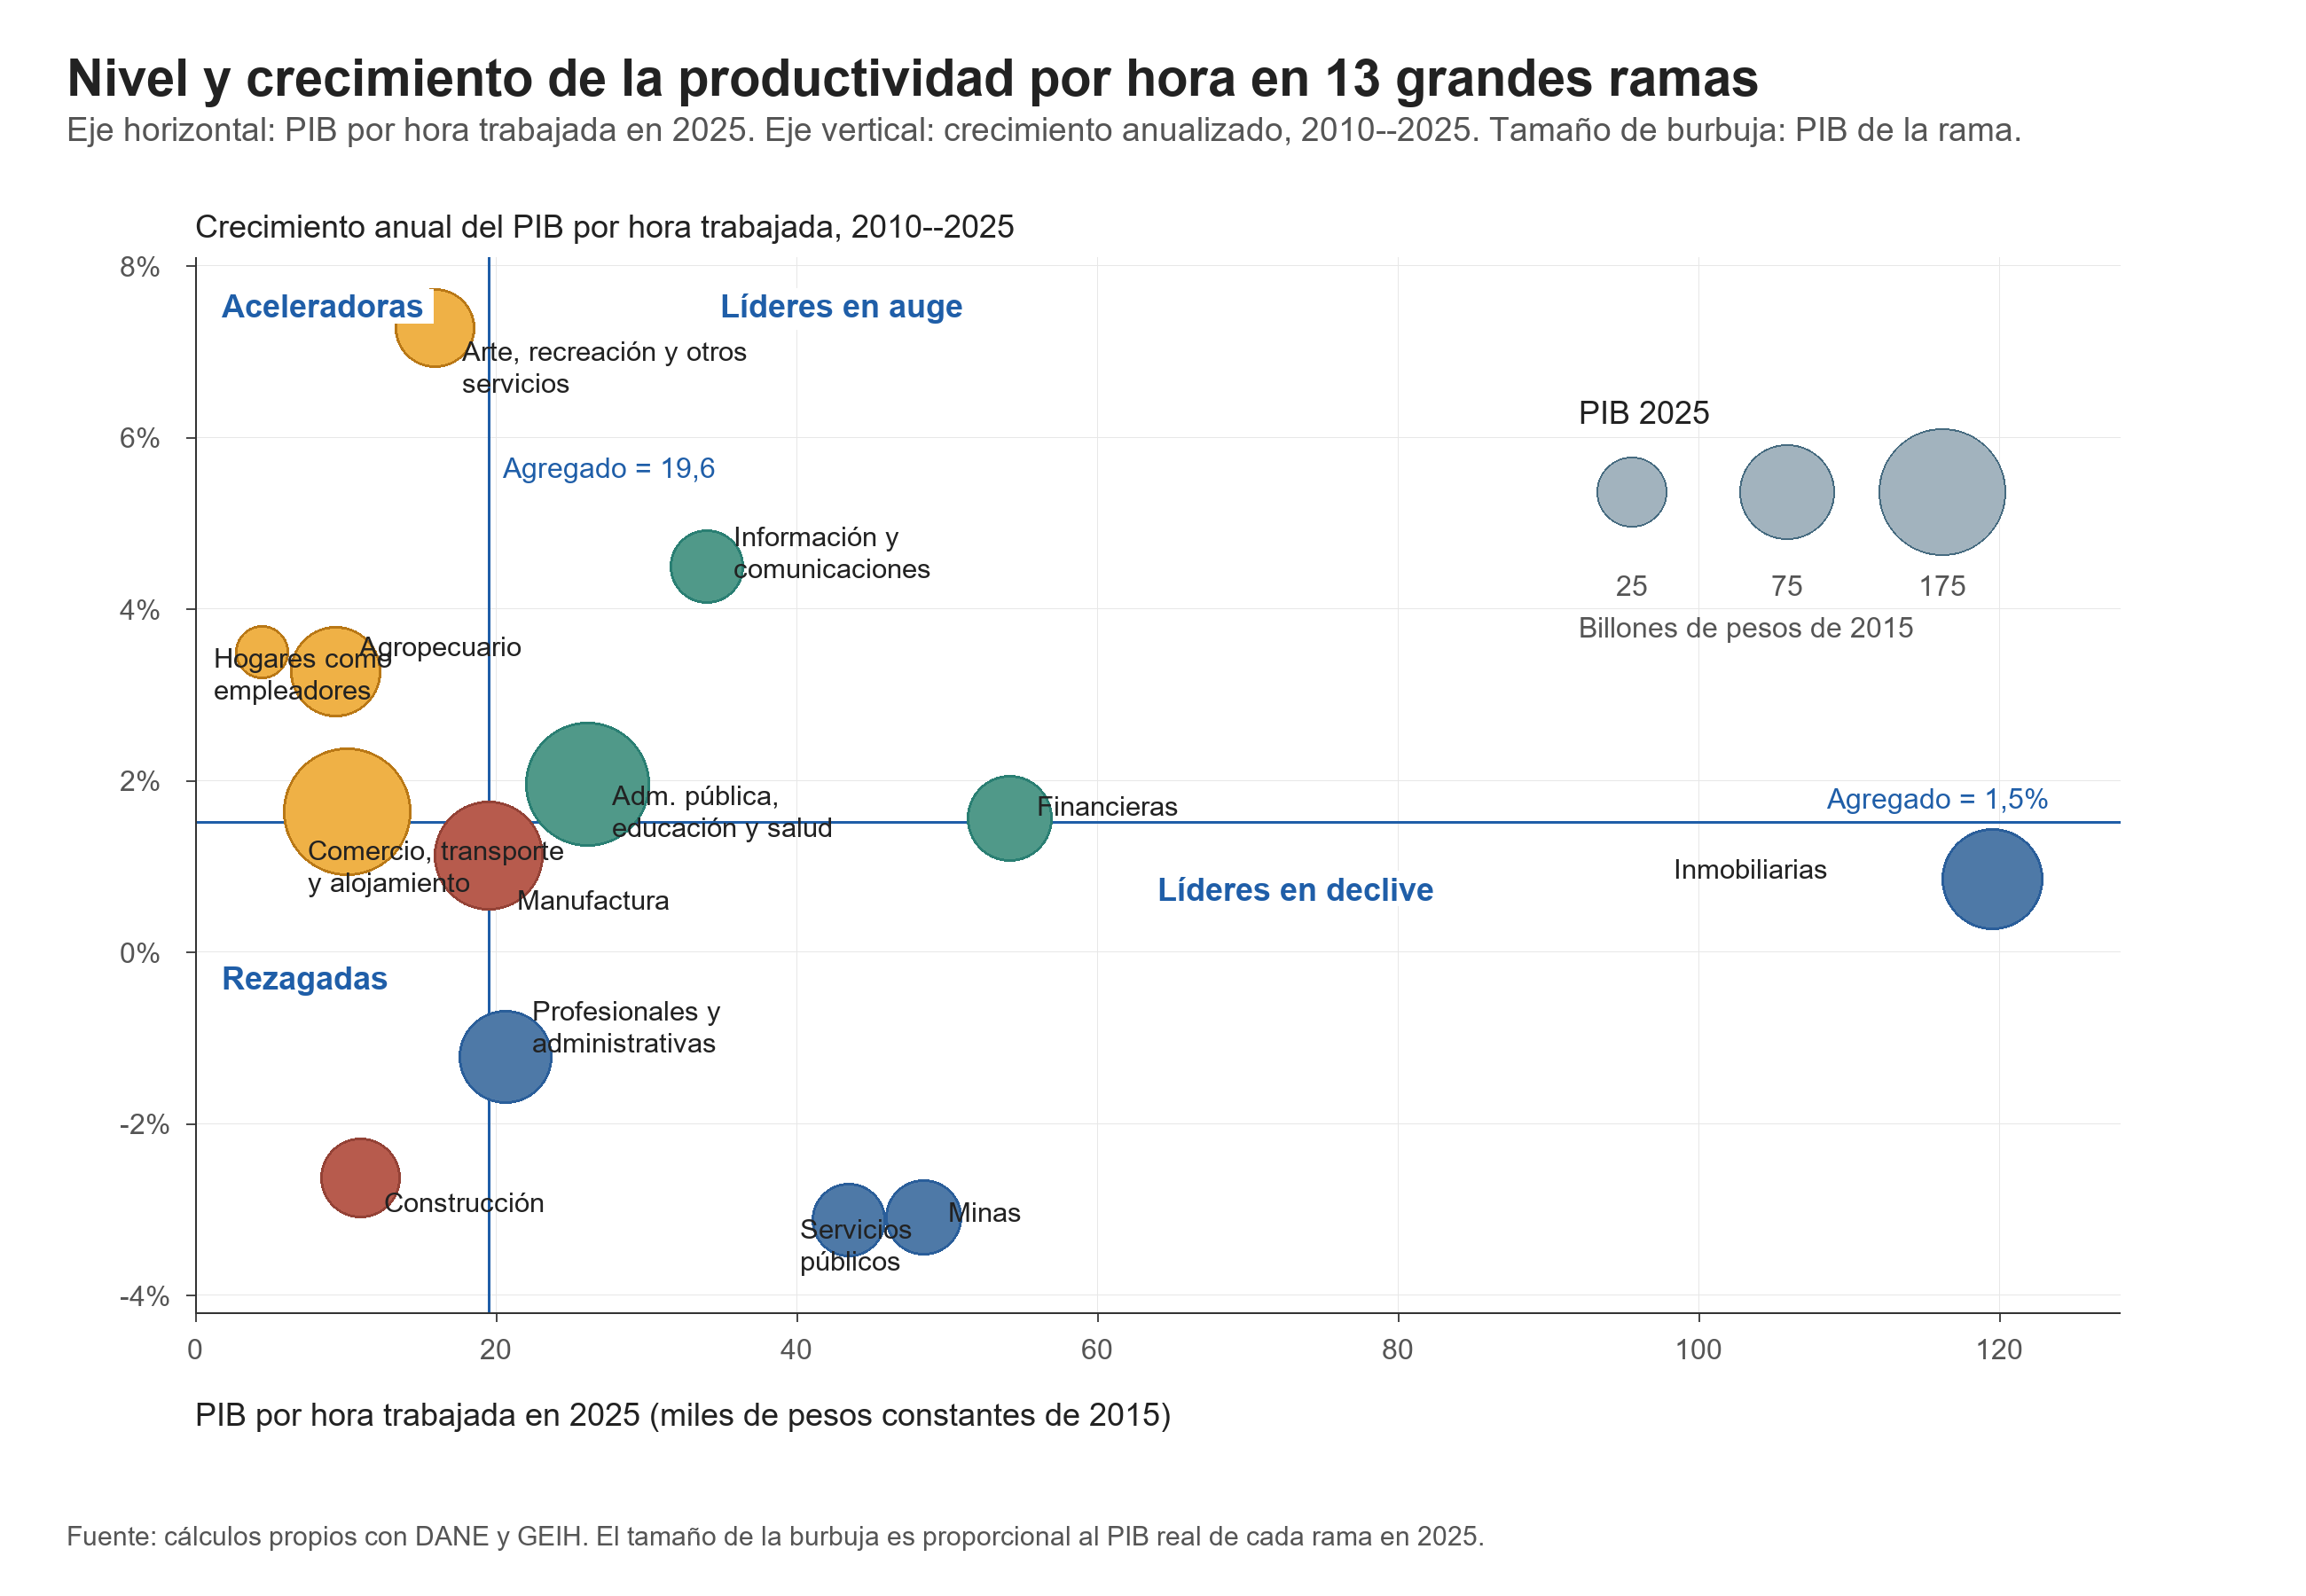
\includegraphics[width=1.21\textwidth,height=0.84\textheight,keepaspectratio]{fig_pib_geih_productividad_burbujas_2025.png}
  \end{center}
\end{frame}

\begin{frame}{Zoom por subactividades}
  \idea{La apertura interna permite ver si el resultado de una gran rama proviene de todas sus subactividades o de algunas en particular.}

  \vspace{0.35cm}
  \begin{itemize}
    \item Los siguientes cuadros presentan la apertura más detallada que puede compararse de manera consistente entre cuentas nacionales y GEIH.
    \item Se muestran solo las ramas donde existe una desagregación laboral comparable.
    \item La lectura combina niveles de productividad en 2025 y crecimiento anual entre 2010 y 2025.
  \end{itemize}
\end{frame}

\begin{frame}{Agropecuario: subactividades}
  \idea{El buen desempeño agropecuario no fue uniforme, pero todas sus subactividades crecieron por encima del agregado.}

  \vspace{0.12cm}
  \begin{center}
  \scriptsize
  \setlength{\tabcolsep}{3.2pt}
  \begin{tabular}{@{}p{0.45\textwidth}rrrr@{}}
    \toprule
    Actividad económica & PIB/trab. 2025 & Crec. & PIB/hora 2025 & Crec. \\
    \midrule
    Silvicultura & 70,2 & 5,15\% & 32,9 & 6,27\% \\
    Pesca y acuicultura & 24,6 & 4,79\% & 10,9 & 5,75\% \\
    Ganadería & 27,1 & 4,45\% & 12,0 & 5,10\% \\
    Cultivos, apoyo agropecuario y mixtos & 20,5 & 2,24\% & 9,6 & 2,61\% \\
    Café & 9,3 & 1,75\% & 4,1 & 1,98\% \\
    \bottomrule
  \end{tabular}
  \end{center}

  \subactividadfuente
\end{frame}

\begin{frame}{Minas: subactividades}
  \idea{La caída de la productividad minera atraviesa casi toda la apertura interna de la rama.}

  \vspace{0.12cm}
  \begin{center}
  \scriptsize
  \setlength{\tabcolsep}{3.2pt}
  \begin{tabular}{@{}p{0.45\textwidth}rrrr@{}}
    \toprule
    Actividad económica & PIB/trab. 2025 & Crec. & PIB/hora 2025 & Crec. \\
    \midrule
    Petróleo, gas y apoyo conexo & 576,1 & 0,07\% & 231,6 & 0,59\% \\
    Otras minas y canteras & 45,6 & -0,89\% & 19,7 & -0,45\% \\
    Carbón & 103,5 & -5,88\% & 41,8 & -5,33\% \\
    Minerales metalíferos & 17,6 & -6,44\% & 7,5 & -5,98\% \\
    \bottomrule
  \end{tabular}
  \end{center}

  \subactividadfuente
\end{frame}

\begin{frame}{Manufactura: subactividades}
  \idea{La manufactura combina subactividades con avances moderados y otras con caídas de productividad.}

  \vspace{0.12cm}
  \begin{center}
  \scriptsize
  \setlength{\tabcolsep}{3.2pt}
  \begin{tabular}{@{}p{0.45\textwidth}rrrr@{}}
    \toprule
    Actividad económica & PIB/trab. 2025 & Crec. & PIB/hora 2025 & Crec. \\
    \midrule
    Metalurgia, maquinaria y equipo & 48,8 & 1,69\% & 20,5 & 2,16\% \\
    Alimentos, bebidas y tabaco & 50,8 & 1,60\% & 21,8 & 1,70\% \\
    Madera, papel e impresión & 46,9 & 1,46\% & 21,8 & 2,21\% \\
    Textiles, confecciones y cuero & 17,5 & 0,74\% & 7,8 & 1,19\% \\
    Refinación, químicos y minerales & 106,6 & -0,75\% & 44,8 & -0,30\% \\
    Muebles y otras manufactureras & 17,4 & -1,38\% & 7,6 & -1,13\% \\
    \bottomrule
  \end{tabular}
  \end{center}

  \subactividadfuente
\end{frame}

\begin{frame}{Servicios públicos: subactividades}
  \idea{La caída de servicios públicos se concentra con especial fuerza en agua, saneamiento y desechos.}

  \vspace{0.12cm}
  \begin{center}
  \scriptsize
  \setlength{\tabcolsep}{3.2pt}
  \begin{tabular}{@{}p{0.45\textwidth}rrrr@{}}
    \toprule
    Actividad económica & PIB/trab. 2025 & Crec. & PIB/hora 2025 & Crec. \\
    \midrule
    Electricidad, gas y vapor & 262,2 & -0,13\% & 109,6 & 0,28\% \\
    Agua, saneamiento y desechos & 37,9 & -6,41\% & 16,9 & -5,74\% \\
    \bottomrule
  \end{tabular}
  \end{center}

  \subactividadfuente
\end{frame}

\begin{frame}{Construcción: subactividades}
  \idea{En construcción, las tres subactividades registraron caídas de productividad.}

  \vspace{0.12cm}
  \begin{center}
  \scriptsize
  \setlength{\tabcolsep}{3.2pt}
  \begin{tabular}{@{}p{0.45\textwidth}rrrr@{}}
    \toprule
    Actividad económica & PIB/trab. 2025 & Crec. & PIB/hora 2025 & Crec. \\
    \midrule
    Obras civiles & 56,2 & -2,58\% & 23,1 & -2,01\% \\
    Actividades especializadas de construcción & 26,7 & -3,27\% & 11,7 & -2,90\% \\
    Edificaciones & 19,9 & -3,52\% & 8,3 & -3,08\% \\
    \bottomrule
  \end{tabular}
  \end{center}

  \subactividadfuente
\end{frame}

\begin{frame}{Comercio, transporte y alojamiento: subactividades}
  \idea{El promedio de esta rama esconde mejores resultados en comercio y rezagos en alojamiento y comida.}

  \vspace{0.12cm}
  \begin{center}
  \scriptsize
  \setlength{\tabcolsep}{3.2pt}
  \begin{tabular}{@{}p{0.45\textwidth}rrrr@{}}
    \toprule
    Actividad económica & PIB/trab. 2025 & Crec. & PIB/hora 2025 & Crec. \\
    \midrule
    Comercio y reparación & 22,8 & 2,28\% & 9,5 & 2,76\% \\
    Transporte y almacenamiento & 27,8 & -0,18\% & 10,9 & 0,83\% \\
    Alojamiento y comida & 23,4 & -1,08\% & 10,7 & -0,42\% \\
    \bottomrule
  \end{tabular}
  \end{center}

  \subactividadfuente
\end{frame}

\begin{frame}{Profesionales y administrativas: subactividades}
  \idea{Las dos subactividades comparables registraron caídas de productividad.}

  \vspace{0.12cm}
  \begin{center}
  \scriptsize
  \setlength{\tabcolsep}{3.2pt}
  \begin{tabular}{@{}p{0.45\textwidth}rrrr@{}}
    \toprule
    Actividad económica & PIB/trab. 2025 & Crec. & PIB/hora 2025 & Crec. \\
    \midrule
    Servicios administrativos y de apoyo & 36,0 & -1,32\% & 18,0 & -0,87\% \\
    Profesionales, científicas y técnicas & 54,7 & -1,91\% & 25,2 & -1,60\% \\
    \bottomrule
  \end{tabular}
  \end{center}

  \subactividadfuente
\end{frame}

\begin{frame}{Adm. pública, educación y salud: subactividades}
  \idea{El crecimiento de esta rama fue favorable, aunque el desempeño por hora no fue igual en sus tres componentes.}

  \vspace{0.12cm}
  \begin{center}
  \scriptsize
  \setlength{\tabcolsep}{3.2pt}
  \begin{tabular}{@{}p{0.45\textwidth}rrrr@{}}
    \toprule
    Actividad económica & PIB/trab. 2025 & Crec. & PIB/hora 2025 & Crec. \\
    \midrule
    Salud y servicios sociales & 49,1 & 2,54\% & 21,3 & 2,47\% \\
    Educación & 52,3 & 1,54\% & 25,8 & 1,26\% \\
    Administración pública & 77,2 & 1,40\% & 32,2 & 2,06\% \\
    \bottomrule
  \end{tabular}
  \end{center}

  \subactividadfuente
\end{frame}

\trayectoriaframe{A}
\trayectoriaframe{B}
\trayectoriaframe{C}
\trayectoriaframe{DE}
\trayectoriaframe{F}
\trayectoriaframe{GHI}
\trayectoriaframe{J}
\trayectoriaframe{K}
\trayectoriaframe{L}
\trayectoriaframe{MN}
\trayectoriaframe{OPQ}
\trayectoriaframe{RS}
\trayectoriaframe{T}

\descomposicionframe{A}
\descomposicionframe{B}
\descomposicionframe{C}
\descomposicionframe{DE}
\descomposicionframe{F}
\descomposicionframe{GHI}
\descomposicionframe{J}
\descomposicionframe{K}
\descomposicionframe{L}
\descomposicionframe{MN}
\descomposicionframe{OPQ}
\descomposicionframe{RS}
\descomposicionframe{T}

\begin{frame}{Ocupación y productividad}
  \idea{Las actividades donde más creció la ocupación no fueron las mismas donde más aumentó la productividad.}

  \vspace{0.1cm}
  \begin{center}
    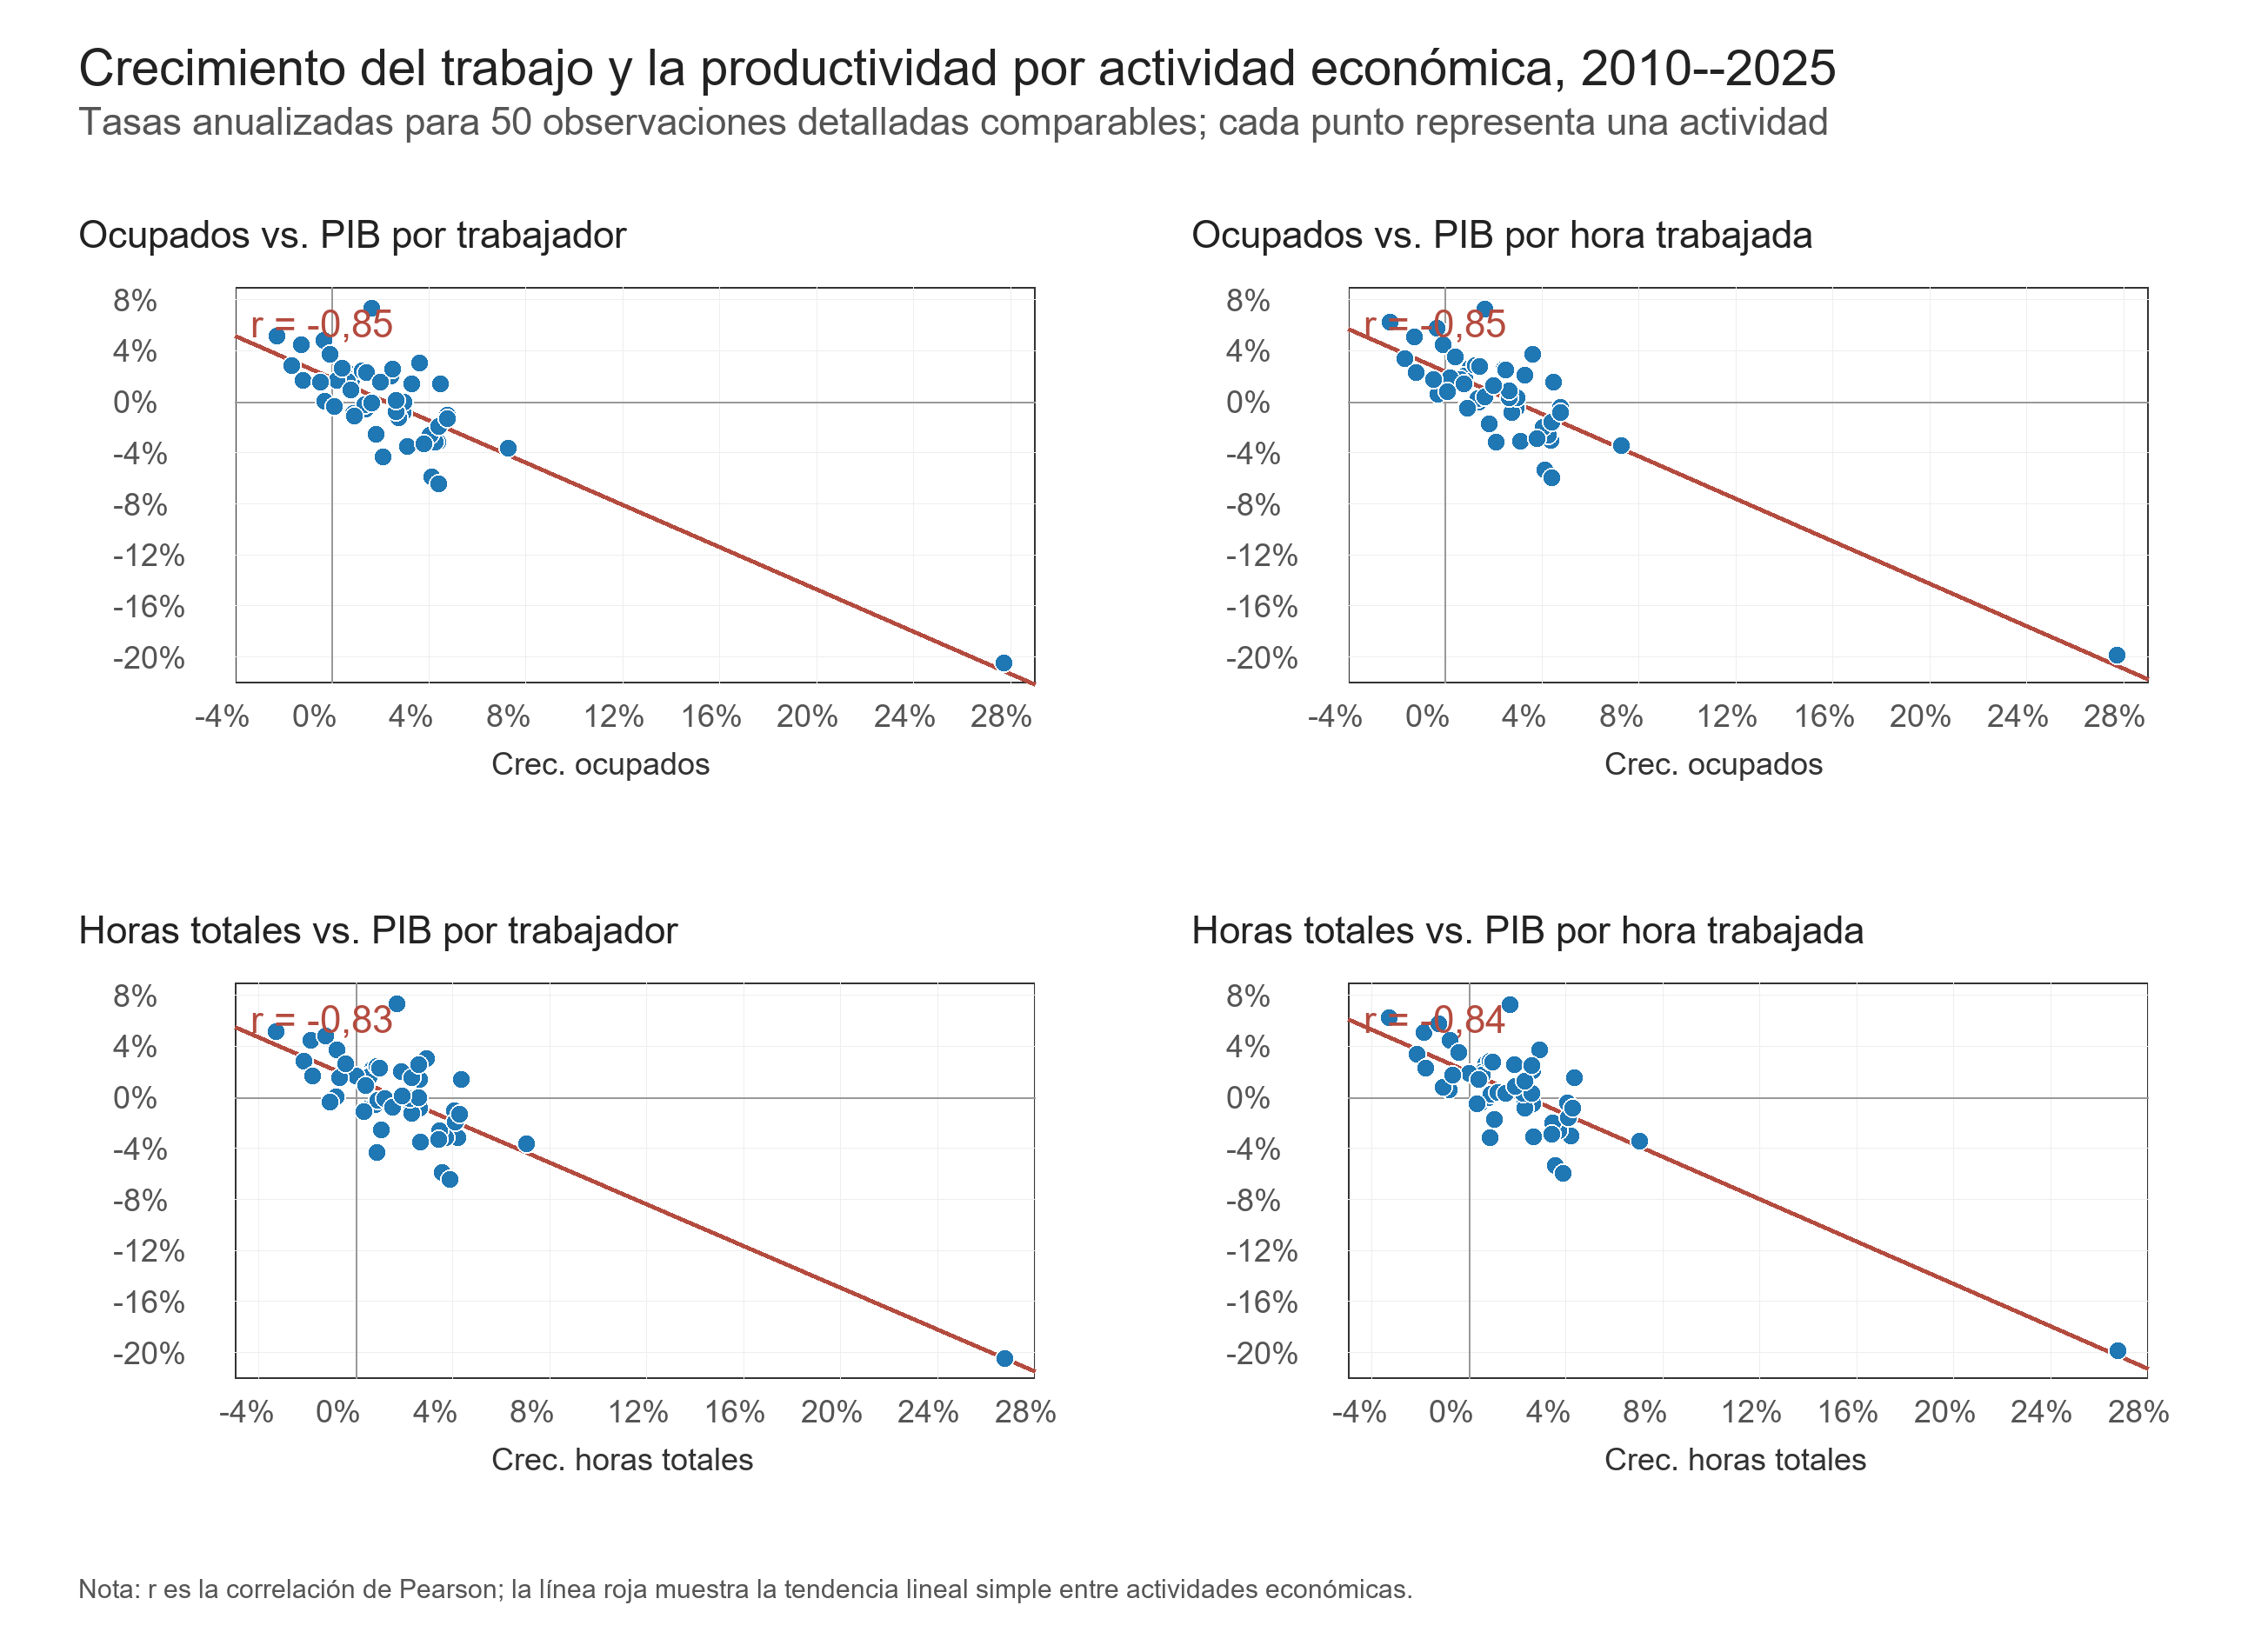
\includegraphics[width=0.88\textwidth,height=0.72\textheight,keepaspectratio]{fig_pib_geih_productividad_sector_correlaciones.png}
  \end{center}

  \fuente{Fuente: cálculos propios con DANE y GEIH.}
\end{frame}

\begin{frame}{Nivel inicial y crecimiento posterior}
  \idea{La evidencia sugiere cierta convergencia: varias actividades con menor productividad inicial crecieron más rápido.}

  \vspace{0.1cm}
  \begin{center}
    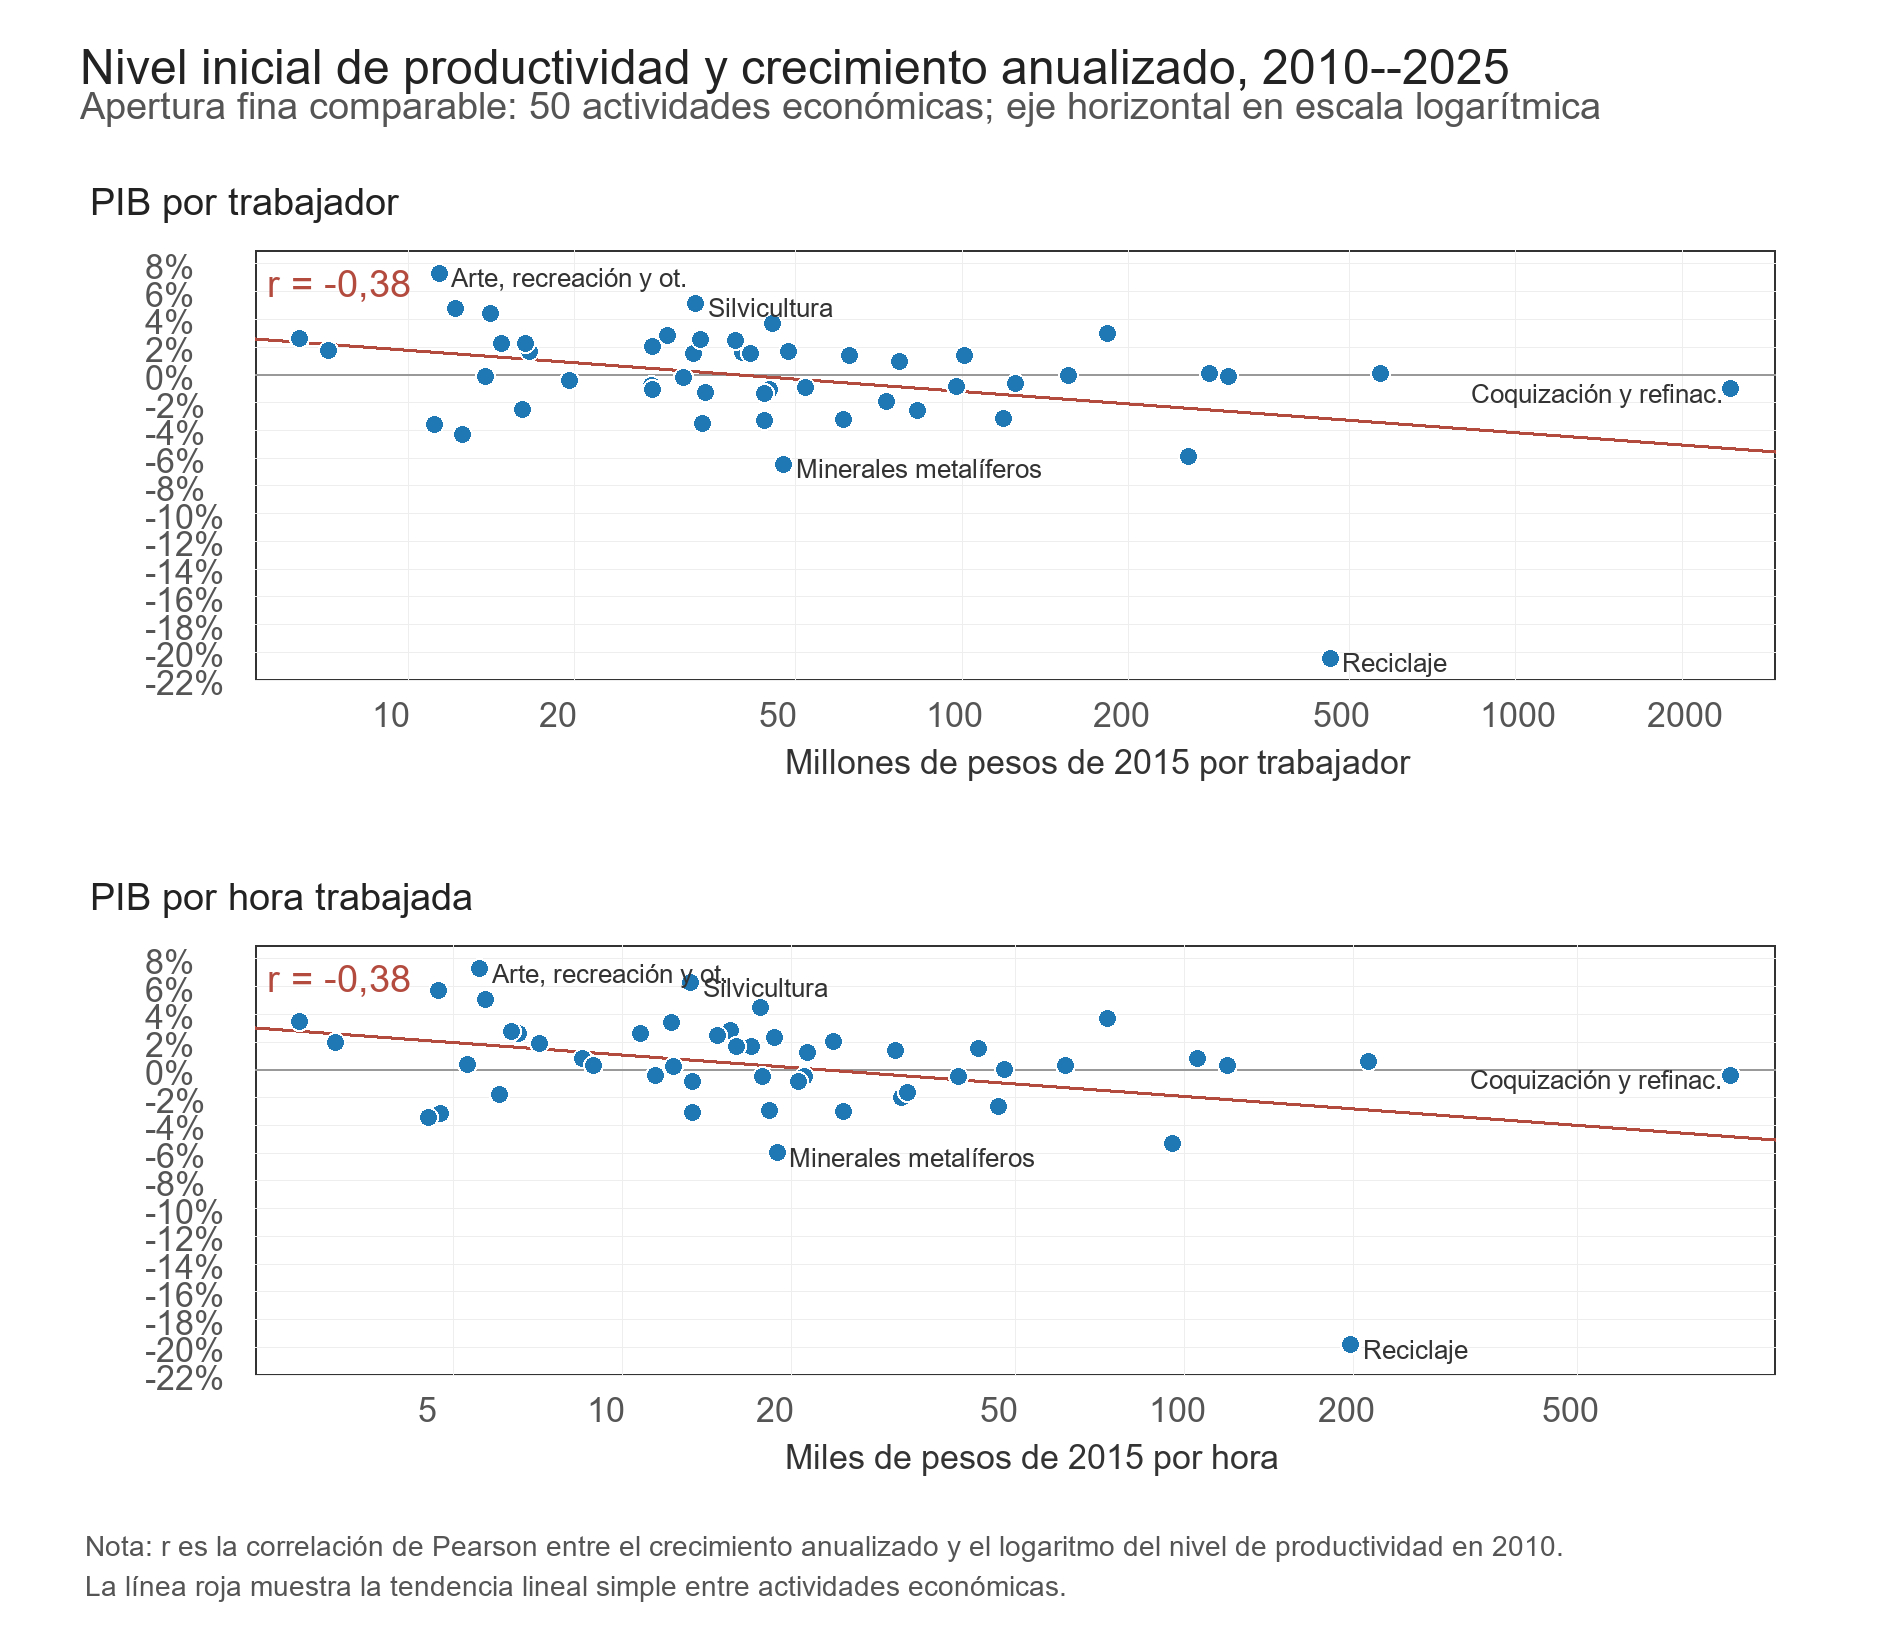
\includegraphics[width=0.88\textwidth,height=0.72\textheight,keepaspectratio]{fig_pib_geih_productividad_nivel_inicial_crecimiento.png}
  \end{center}

  \fuente{Fuente: cálculos propios con DANE y GEIH.}
\end{frame}

\begin{frame}{Conclusiones}
  \idea{El crecimiento de la productividad debe convertirse en una prioridad de la agenda económica nacional.}

  \vspace{0.35cm}
  \begin{itemize}
    \item Colombia creció más por aumento de ocupados que por aumento del producto por trabajador.
    \item La productividad por hora creció más rápido que la productividad por trabajador porque las horas trabajadas por ocupado cayeron.
    \item La mirada por actividad económica muestra un panorama muy desigual: algunas actividades avanzaron con fuerza y otras redujeron su productividad.
    \item La agenda del país debe identificar dónde se está frenando la productividad y qué condiciones permitirían extender las mejoras al resto de la economía.
  \end{itemize}
\end{frame}

\end{document}
